\documentclass{article}
\usepackage[
        a4paper,% other options: a3paper, a5paper, etc
        left=3cm,
        right=3cm,
        top=3cm,
        bottom=4cm,
        % use vmargin=2cm to make vertical margins equal to 2cm.
        % us  hmargin=3cm to make horizontal margins equal to 3cm.
        % use margin=3cm to make all margins  equal to 3cm.
]{geometry}
%\usepackage[utf8x]{inputenc}
\usepackage{graphicx}
\usepackage{caption}
\usepackage{enumerate}
\usepackage{subcaption}
\usepackage[procnames]{listings}
\usepackage{color}
\usepackage{amssymb}
\usepackage{amsmath}
\usepackage{amsfonts}
\usepackage{comment}
\usepackage{hyperref}
\usepackage{blindtext}
\usepackage[scaled=.8]{sourcecodepro}
\setcounter{section}{+1}
\definecolor{codegreen}{rgb}{0,0.6,0}
\definecolor{codegray}{rgb}{0.5,0.5,0.5}
\definecolor{codepurple}{rgb}{0.58,0,0.82}
\definecolor{backcolour}{rgb}{0.95,0.95,0.92}
 
%\renewcommand*\ttdefault{pcr} 
 
\lstdefinestyle{mystyle}{
    backgroundcolor=\color{backcolour},   
    commentstyle=\color{codegreen},
    keywordstyle=\color{blue},
    numberstyle=\tiny\color{codegray},
    stringstyle=\color{codepurple},
    basicstyle=\ttfamily,
    breakatwhitespace=false,         
    breaklines=true,                 
    captionpos=b,                    
    keepspaces=true,                 
    numbers=left,                    
    numbersep=5pt,                  
    showspaces=false,                
    showstringspaces=false,
    showtabs=false,                  
    tabsize=2
}

\title{Lab Assignment 4\\ {\Large Convolutional Neural Networks}}
\date{\today}
\author{
 	Eleftherios Karamoulas - S3261859\\ 
	Panagiotis Tzafos - S3302148\\
}

\lstset{style=mystyle, language=Matlab}
\begin{document}
\maketitle
\section{Theory questions}
\begin{enumerate}
\item The pooling layer serves to progressively reduce the spatial size of the representation, to reduce the number of parameters and amount of computation in the network, and hence to also control overfitting(CS231n lecture). In practice, its use is to downsample its input, reducing the amount of resources that the network needs in order to perform the computations by reducing the dimensions of the input using a filter, a stride and an elementwise activation function. Also, after the downsampling it is obvious that the network will have less parameters. As a result, it will be able to generalize better in new situations and avoid overfitting(small training set error, large error for new examples). 
\item
Weight sharing is a very important feature, as it can dramatically reduce the number of weights(less computations). The idea behind this is that the number of unique sets of weights can be equal to the number of filters that are going to be used, as we are about use these to every different region of the image we are scanning. This is when the network is interested to examine if a feature exists in the image indepentantly by its position. It can be applied because of the fact that, assuming that a single depth slice(filter) weight configuration is associated with a single feature that our network is looking for(edges, circles etc.), in every single one spatial region that the filter checks, it responsible of tracing these specific features(Not useful when the network has to learn in different positions of the image different features, e.g. a training set of faces, that are centralized). 
\item
The time is less in ReLu activation function compared to the sigmoid and the tanh activation functions, as it does not involve expensive operations(exponentials, etc.), as it can be implemented by simply thresholding a matrix of activations at zero. The results are better because of the properties that ReLu function provides, like sparse representation(the more activations are \(\le 0 \) the more sparse is our model and this is generally more beneficial than dense representations that sigmoid and tanh provide) and ReLu function non-saturating form(sigmoid and tanh functions are vanishing gradient, as the absolute value of x in \(\alpha = Wx + b \) increases the gradient of sigmoid becomes increasingly small compared to ReLu that the gradient is constant.) 
\item 
\begin{enumerate}
\item From the given data and the formula to compute the output we have that \(W=12, F=3, P=0, S=1\), so output \(= \frac{W - F + 2 * P}{S}+1 = \frac{12 - 3 + 2 * 0}{1}+1=  10\) and because we have 3 filters the total neurons will be 10 x 10 x 3 = 300. The total number of parameters will be 300 x 1 weights for the full depth(grayscale) of the input image + 3 for the 3 biases of each filters = 303.\\
\item
 The input layer is our image and if we assume that each pixel is one neuron, our input layer consists of 12 x 12 = 144 neurons and each of them will be fully connected to our neurons in the hidden layer which consists of 300 neurons. As a result the total connections between input and hidden layer will be 144 x 300 = 43200 weights + 300 biases = 43500. It is obvious that the number of parameters of the fully-connected layer compared with a convolutional layer is much bigger, and that makes convolutional layer more efficient. \\
\end{enumerate}
\item This approach to solve the car decision problem is questionable because even though we can use CNN's and get a network that can decide between cars an average solution, the features that characterise the car can be subjective for different customers depending on their needs and comforts.
\end{enumerate}
\setcounter{section}{+3}
\section{Convolutional Layer}
\lstinputlisting[caption={cnnConvolve.m},label={code:bar}]{cnn/cnnConvolve.m}
\section{Mean Pooling Layer}
\lstinputlisting[caption={cnnPool.m},label={code:bar}]{cnn/cnnPool.m}
\section{Forward Pass}
\lstinputlisting[caption={cnnCost.m},label={code:bar}]{cnn/cnnCost.m}
\section{Experiments}
\begin{enumerate}
\item Our network starts with the imageDim parameter that its the input image dimension(W), creating a matrix imageDim x imageDim. The parameter numClasses is the output of the network, that basically is a vector numClasses x 1, that contains the possibilities that our input is associated with one of these classes(e.g. 10 digits 1 class for each, the sum of the possibilities must be equal to 1, the biggest possibility is the class that our input is associated). The parameter filterDim is the filter dimension. More specifically, this is responsible for creating a square filter with dimensions filterDim x filterDim x imageDepth (imageDepth = 3 for RGB, = 1 for Grayscale, every neuron is connected with a part-filter on the image, using the full image Depth), that we are using for iteratings over the different spatial region of the image. The numFilters parameters is the number of different features we are looking for in each different spatial region of the image, using our filters. The parameter poolDim is responsible for downgrading the output volume, e.g. for poolDim 2 in an output volume 28 x 28 x numFilters, we will have a 14 x 14 x numFilters result as new output volume. In our example, we are using batch combined with stochastic gradient training, as we are not using all the training set at once(batch), but neither every single training set example alone. Instead we are using small batches of images for training. Our cnnConvolve function is responsibe for the output volume, so every output of this function is the activation-output volume for a specific batch of images, all the filters applied in each and its structure is outputVolumeDim(imageDim - filterDim + 1) x outputVolumeDim x numFilters x numImages(Images for the current batch). After these, we are passing this matrix as a parameter to our pooling layer, in order to downgrade the image. Then we are reshaping, the first three dimensions into a continuous vector for each image, so now we have a two dimensional matrix, that contains the data for each image. Last step of forward passing is computing the propabilities for each image(which class is associated with each image more). Softmax layer is responsible for this, as it is using the current weight matrix, the biases and the input vector for each image to calculate the result. After this we are calculating the cost, and we proceed to the back propagation, in order to continue our network training. Using the built-in minFuncSGD matlab function, we are passing as parameters our cost function(cnnCost.m) with the rest of the network parameters, and we are using as option 3 epochs with batches of 256 images and a learning rate of 1e-1. After these steps, we are testing our accuracy(answer at 7.3 about the results). The procedure of learning and testing is finished.
\item In the beginning of the training we see that our filters look like random noise patches but as our training progresses we see that the filters achieve more structure and finally after 3 epochs we can see clearly on them shapes e.g.(lines, angles, curves) that they can recognize on images that we feed to our network.
\begin{figure}[!h]
    \centering
    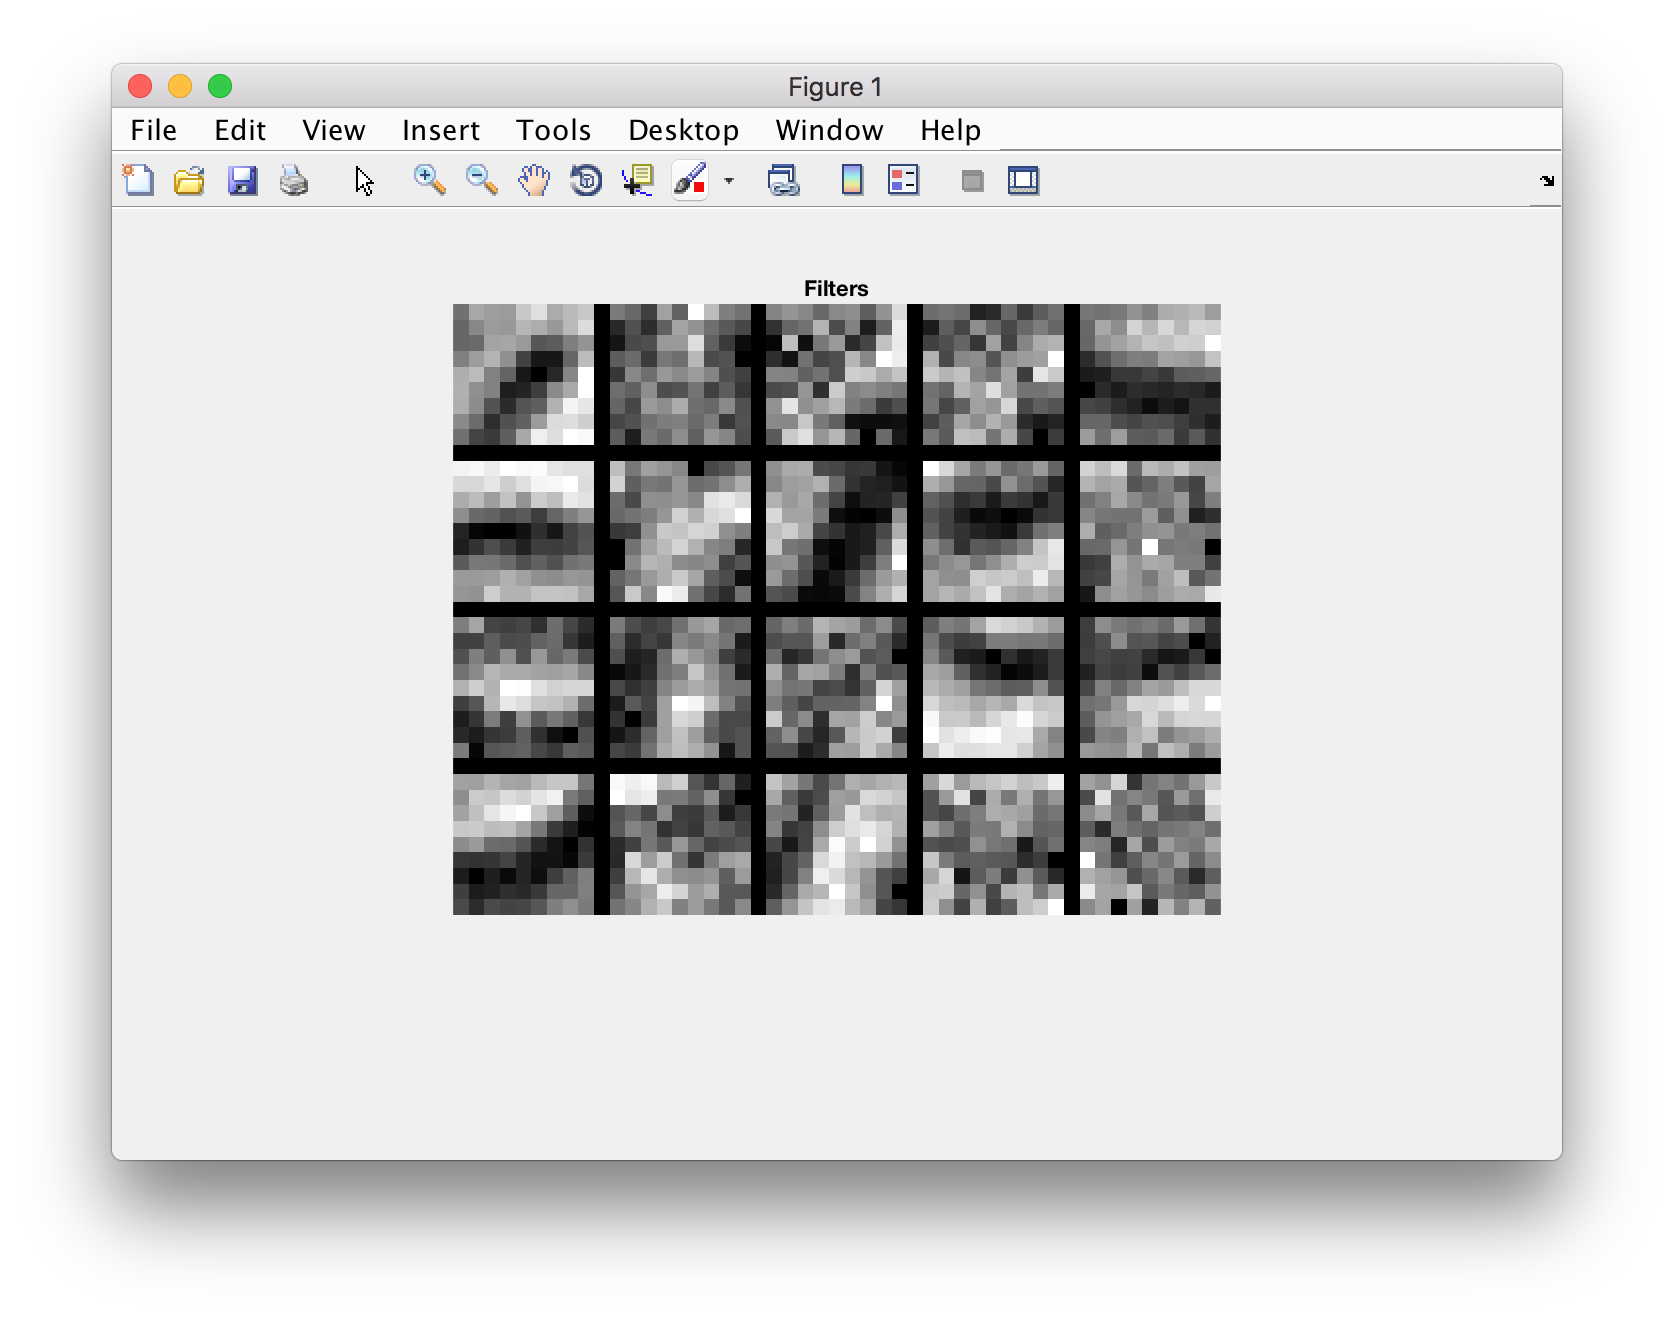
\includegraphics[width=1\textwidth]{filters.png}
    \caption{Filters after 3 epochs}
    \label{fig:picture}
  \end{figure}
\item Our network accuracy after 3 epochs is 97.24\%
\end{enumerate}
\end{document}
